\documentclass[runningheads]{llncs}
\usepackage{graphicx}
\usepackage{float}
\usepackage{hyperref}
\usepackage[style=ieee,citestyle=numeric-comp,dashed=false]{biblatex}
\usepackage{booktabs}
\usepackage{multirow}
\usepackage{todonotes}
\addbibresource{refs.bib}

\begin{document}
\title{Finding Code Clone Refactoring Techniques by Mapping Clone Context}

\author{Simon Baars\inst{1,2}\orcidID{0000-0001-7905-1027} \and
Ana Oprescu\inst{1,3}\orcidID{0000-0001-6376-0750}}

\institute{University of Amsterdam \and
\email{simon.j.baars@gmail.com} \and
\email{A.M.Oprescu@uva.nl}}
\maketitle

\begin{abstract}
Reducing clones in source code is one of the techniques to improve the maintainability of a software system. Which refactoring technique to use depends on where a clone is found and what the relation between clone instances in a clone class is. We define three influencing factors on how a clone should be refactored: relation, location and contents. The relation describes the inheritance relation among the clone instances in a clone class. The location describes where a clone instance is found in the source code. The contents describe what a clone instance spans.

Based on experiments on corpus of open-source Java projects we find that most clones (77\%) are in the body of methods or constructors and thus the ``Extract Method'' refactoring technique applies. What further techniques are required for the refactoring depends on the relation among the clone instances of a clone. We define four relations that require different further refactoring techniques: Common Class, Common Hierarchy, Common Interface and Unrelated. The closer classes are related, the more favorable refactoring clones by such relations becomes. 37\% of clones are in the same class, 24\% share an inheritance hierarchy, 24\% are unrelated and 15\% have a common interface.

\keywords{Code Clones \and Mining Software Repositories \and Clone Relation \and Inheritance \and Object-Oriented Programming.}
\end{abstract}

\section{Introduction}
Duplicate code fragments are often considered as bad design~\cite{fowler2018refactoring}. They increase maintenance efforts or cause bugs in evolving software~\cite{heitlager2007practical}. Changing one occurrence of a duplicated fragment may require changes in other occurrences~\cite{ostberg2014automatically}. Furthermore, duplicated code was shown to account for up to 25\% of total system volume~\cite{bruntink2005use}, entailing more code to be maintained.

Several refactoring techniques can be used to reduce duplication in source code~\cite{fowler2018refactoring}. Which refactoring technique to apply depends on where a clone is located and what the relation is between similar code fragments \cite{koni2001scenario}. Subsequent studies have performed statistical measurements on how many clones fall into these location and relation categories \cite{fontana2012duplicated, fontana2015duplicated}.

We extend the state-of-the-art \cite{fontana2015duplicated} by defining location, relation and contents categories for clones to determine how they should be refactored. The extra categories we provide help to propose a refactoring opportunity that can automatically be applied, rather than merely suggesting the technique that has to be used \cite{fontana2015duplicated}.

We study a large corpus of open-source software systems to determine which relation, location and contents category has the most clones. We find that a significant portion of clones is found in the bodies of constructors and methods, which indicate clones that can be refactored by applying the ``Extract Method'' refactoring technique. What further techniques apply when refactoring such a clone depends on the relation among its clone instances.

If clone instances share a common class, no further refactoring techniques are required. If they are in the same inheritance hierarchy, the ``Pull-Up Method'' can be used till the extracted method is in a location accessible by all instances. If the instances share a common interface, some languages allow to move the extracted method there. Otherwise, if the clone instances are not related, we either have to create a superclass/interface abstraction or create a utility class to put the common functionality.

\section{Background and Related Work}
We use two definitions to argue about code clones~\cite{roy2007survey}:
\begin{itemize}
    \item \textbf{Clone instance}: A single code fragment of which a similar/identical copy exists elsewhere in the codebase.
    \item \textbf{Clone class}: A set of similar/identical clone instances.
\end{itemize}

To argue about the similarity relation between clone instances in a clone class, several clone type definitions have been proposed~\cite{roy2007survey}:
\begin{itemize}
    \item \textbf{Type 1:} Identical code fragments except for variations in whitespace (may also be variations in layout) and comments.
    \item \textbf{Type 2:} Structurally/syntactically identical fragments except for variations in identifiers, literals, types, layout and comments.
    \item \textbf{Type 3:} Copied fragments with further modifications. Statements can be changed, added or removed in addition to variations in identifiers, literals, types, layout, and comments.
\end{itemize}

A higher type of clone means that it is harder to detect. It also makes the clone harder to refactor, as more transformations would be required. Higher clone types also become more disputable whether they actually indicate a harmful anti-pattern as not every clone is harmful~\cite{jarzabek2010clones, kapser2008cloning}.

Next, we outline relevant research to clone refactoring. A significant aspect is the context of clones.

\subsection{Clone context analysis}\label{sec:rw:contextanalysis}
Golomingi~\cite{koni2001scenario} explores mapping the relation between clone instances to refactoring methods. The author analyses the refactoring methods described by Martin Fowler~\cite{fowler1999refactoring} and analyzes what refactoring methods can be used to refactor clones with what inheritance relations. The identified clone relations are: Ancestor, Common Hierarchy, First Cousin, Same Method, Sibling, Single Class, Superclass and Unrelated. We extend this list with several more fine-grained relations, suitable for automatic refactoring.

Fontana et al.~\cite{fontana2012duplicated, fontana2015duplicated} combine the research by Golomingi~\cite{koni2001scenario} with clone types 1 and 3 \cite{roy2007survey}. They use a large corpus~\cite{tempero2010qualitas} on which they perform statistical analysis of clone relations together with clone types. We repeat this research with a different setup, namely we elaborate further in the categories analysed, and thus get results with a finer granularity, and we use a larger dataset, namely the GitHub set of repositories~\cite{githubCorpus2013}. 

\subsection{Clone refactoring}
Krishnan et al.~\cite{krishnan2013refactoring} approach clone refactoring as an optimization problem: how variability between cloned fragments influences the refactoring techniques required and their implications on system design. The main focus of this study is to find out which clones \textbf{can} be refactored. We extend this work by looking into which clones \textbf{should} be refactored. We propose definitions for refactorable clones together with thresholds to be able to limit their negative impact on system design. We measure which clones improve maintainability when refactored. This results in a set of thresholds that can be used to detect and refactor clones that should be refactored.

For refactoring clones, we took naming the extracted method outside of the scope of the study. To have this not influence the results, the metrics that determine the maintainability of an applied refactoring do not measure the quality of the name of the extracted method. 

\section{Context Analysis of Clones}\label{chap:contextsetup}
The context of a clone determines how it should be refactored~\cite{fowler2018refactoring}. Based on current literature \cite{fontana2012duplicated, fontana2015duplicated}, we define the following aspects of a clone as its context:
\begin{itemize}
  \item \textbf{Relation:} The relation of clone instances in a clone class through inheritance.
  \item \textbf{Location:} Where a clone instance occurs in the code.
  \item \textbf{Contents:} The statements/declarations of a clone instance.
\end{itemize}

\subsection{Relation}\label{sec:setuprelation}
When merging code clones in object-oriented languages, it is important to consider the relation between clone instances. This relation has a big impact on how a clone should be refactored.

Fontana et al.~\cite{fontana2015duplicated} describe measurements on 50 open source projects on the relation between clone instances in a clone class. To do this, they first define several categories to argue about such relations. These categories are as follows:
\begin{itemize}
  \item \textbf{Same Method}: All instances of the clone class are in the same method.
  \item \textbf{Same Class}: All instances of the clone class are in the same class.
  \item \textbf{Superclass}: All instances of the clone class are in a class that are child or parent of each other.
  \item \textbf{Sibling Class}: All instances of the clone class have the same parent class.
    \item \textbf{Ancestor Class}: All instances of the clone class are superclasses except for the direct superclass.
  \item \textbf{First Cousin Class}: All instances of the clone class have the same grandparent class.
    \item \textbf{Same Hierarchy Class}: All instances of the clone class belong to the same inheritance hierarchy, but do not belong to any of the other categories.
\item \textbf{Same External Superclass}: All instances of the clone class have the same superclass, but this superclass is not included in the project but part of a library.
\item \textbf{Unrelated class}: There is at least one instance of the clone class that is not in the same hierarchy.
\end{itemize}

We added the following categories, to gain more information about clones and be able to suggest a more fine-grained refactoring opportunity:

\begin{itemize}
\item \textbf{Same Direct Interface}: All instances of the clone class are in a class or interface implement the same interface.
\item \textbf{Same Indirect Interface}: All instances of the clone class are in a class or interface that have a common interface anywhere in their inheritance hierarchy.
\item \textbf{No Direct Superclass}: All instances of the clone class are in a class that does not have any superclass.
\item \textbf{No Indirect Superclass}: All instances of the clone class are in a class that does not have any external classes in its inheritance hierarchy.
\item \textbf{External Ancestor}: All instances of the clone class are in a class that does not have any external classes in its inheritance hierarchy.
\end{itemize}

\begin{figure}
  \centering
    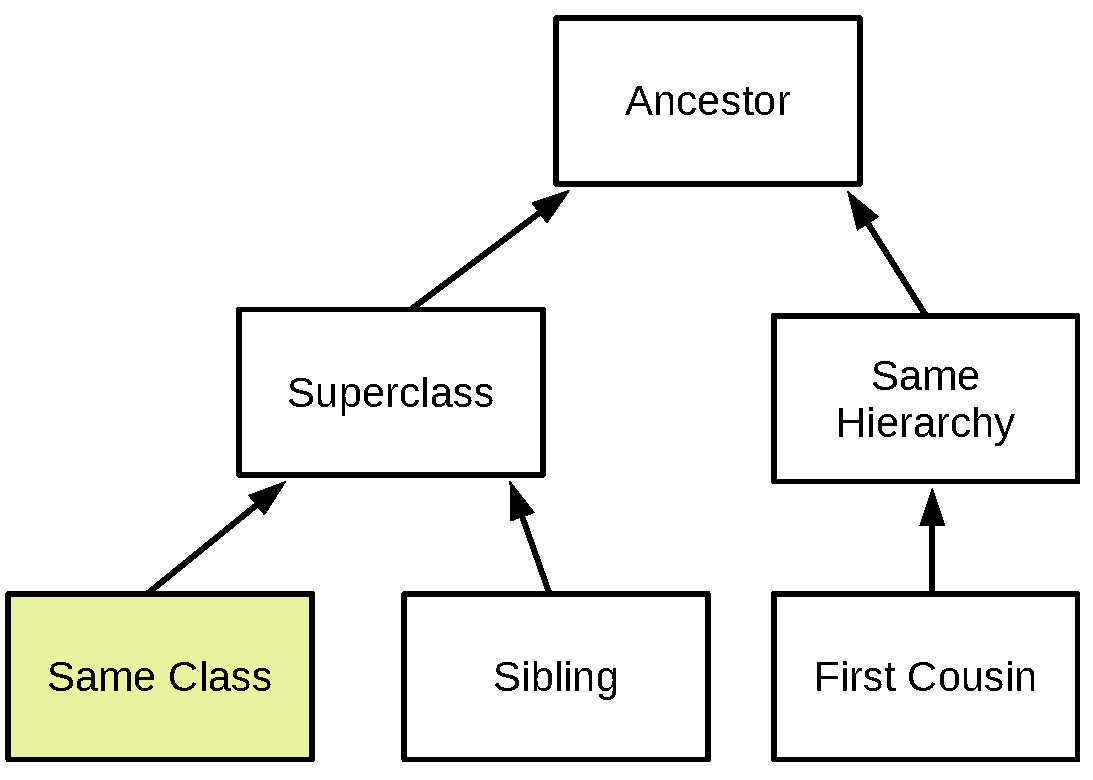
\includegraphics[width=0.6\columnwidth]{img/Relation}
      \caption{Abstract figure displaying some relations of clone classes. Arrows represent superclass relations.}
  \label{fig:clonerelation}
\end{figure}

We separate these relations into the following categories, because of their related refactoring opportunities:
\begin{itemize}
  \item \textbf{Common Class}: \textit{Same Method}, \textit{Same Class}
  \item \textbf{Common Hierarchy}: \textit{Superclass}, \textit{Sibling Class}, \textit{Ancestor Class}, \textit{First Cousin}, \textit{Same Hierarchy}
  \item \textbf{Common Interface}: \textit{Same Direct Interface}, \textit{Same Indirect Interface}
  \item \textbf{Unrelated}: \textit{No Direct Superclass}, \textit{No Indirect Superclass}, \textit{External Superclass}, \textit{External Ancestor}
\end{itemize}

Every clone class only has a single relation, which is the first relation from the above list that the clone class applies to. For instance: all ``Superclass'' clones also apply to ``Same Hierarchy'', but because ``Superclass'' is earlier in the above list they will get the ``Superclass'' relation. This is because the items earlier in the above list denote a more favorable refactoring.


\subsubsection{Common Class}
The \textit{Same method} and \textit{Same class} relations share a common refactoring opportunity. Clones of both these categories, when extracted to a new method, can be placed in the same class. Both of these relations are most favorable for refactoring, as they require a minimal design tradeoff. Furthermore, global variables that are used in the class can be used without having to create method parameters.


\subsubsection{Common Hierarchy}
Clones that are in a common hierarchy can be refactored by using the ``Extract Method'' refactoring method followed by ``Pull Up Method'' until the method reaches a location that is accessible by all clone instances. However, the more often ``Pull Up Method'' has to be used, the more detrimental the effect is on system design. This is because putting a lot of functionality in classes higher up in an inheritance structure can result in the ``God Object'' anti-pattern. A god object is an object that knows too much or does too much~\cite{fowler2018refactoring}.


\subsubsection{Common Interface}
Many object-oriented languages know the concept of ``interfaces'', which are used to specify a behavior that classes must implement. As code clones describe functionality and interfaces originally did not allow for functionality, interfaces did not open up refactoring opportunities for duplicated code. However, many programming languages nowadays support default implementations in interfaces. Since Java 7 and C\# 8, these programming languages allow for functionality to be defined in interfaces. Many other object-oriented languages like Python allow this by nature, as they do not have a true notion of interfaces.

The greatest downside on system design of putting functionality in interfaces is that interfaces are per definition part of a classes' public contract. That is, all functionality that is shared between classes via an interface cannot be hidden by stricter visibility. Because of that, we favor all ``Common Hierarchy'' refactoring opportunities over ``Common Interface''.


\subsubsection{Unrelated}
Clones are unrelated if they share no common class or interface in their inheritance structure. These clones are least favorable for refactoring, because their refactoring will almost always have a major impact on system design. We formulated four categories of unrelated clones to look into their refactoring opportunities.

Cloned classes with a \textit{No Direct Superclass} relation mark the opportunity for creating a superclass abstraction and placing the extracted method there. For clone classes with a \textit{No Indirect Superclass} relation, it is possible to create such an abstraction for the ancestor that does not have a parent. Clone classes with an \textit{External Superclass} or \textit{External Ancestor} relation obstruct the possibility of creating a superclass abstraction. In such a case, it is possible to create an interface abstraction to make their relation explicit.


\subsection{Location}\label{sec:setuplocation}
A paper by Lozano et al.~\cite{lozano2007evaluating} discusses the harmfulness of cloning. The authors argue that 98\% are produced at method-level. However, this claim is based on a small dataset and based on human copy-paste behavior rather than static code analysis. We decided to measure the locations of clones through static analysis in our dataset. We chose the following categories:
\begin{itemize}
  \item \textbf{Method/Constructor Level:} A clone instance that does not exceed the boundaries of a single method or constructor (optionally including the declaration of the method or constructor itself).
  \item \textbf{Class Level:} A clone instance in a class, that exceeds the boundaries of a single method or contains something else in the class (like field declarations, other methods, etc.).
  \item \textbf{Interface/Enumeration Level:} A clone that is (a part of) an interface or enumeration.
\end{itemize}
We check the location of each clone instance for each of its nodes. If any node reports a different location from the others, we choose the location that is lowest in the above list. So for instance, if a clone instance has 15 nodes that denote a \textit{Method Level} location but 3 nodes are \textit{Class Level}, the clone instance becomes \textit{Class Level}.

\subsubsection{Method/Constructor Level Clones} \label{sec:methodlevelcr}
Method/Constructor Level clones denote clones that are found in either a method or constructor. A constructor is a special method that is called when an object is instantiated. Most modern clone refactoring studies only focus on clones at method level~\cite{yue2018automatic, yongting2018detection}. This is because most clones reside at those places~\cite{lozano2007evaluating, fontana2015duplicated} and most of those clones can be refactored with a relatively simple set of refactoring techniques~\cite{kodhai2013method, fontana2015duplicated}.


\subsubsection{Class/Interface/Enumeration Level Clones}
Class/Interface/Enumeration Level clone instances are found inside the body of one of these declarations and optionally include the declaration itself. It can also be a clone instance that exceeds the boundaries of a single method. These clone instances can contain fields, (abstract) methods, inner classes, enumeration fields, etc. These types of clones require various refactoring techniques to refactor. For instance, we might have to move fields in an inheritance hierarchy. Or, we might have to perform refactoring on an architectural level, if a large set of methods is cloned.


\subsection{Contents}\label{sec:setupcontents}
Finally, we looked at what nodes individual clone instances span. We selected a set of categories based on empirical evaluation of a set of clones in our dataset. We selected the following categories to be relevant for refactoring:
\begin{itemize}
  \item \textbf{Full Method/Constructor/Class/Interface/Enumeration:} A clone that spans a full class, method, constructor, interface or enumeration, including its declaration.
  \item \textbf{Partial Method/Constructor:} A clone that spans (a part of) the body of a method/constructor. The declaration itself is not included.
  \item \textbf{Several Methods:} A clone that spans over two or more methods, either fully or partially, but does not span anything but methods (so not fields or anything in between).
  \item \textbf{Only Fields:} A clone that spans only global variables.
  \item \textbf{Other:} Anything that does not match with above-stated categories.
\end{itemize}

\subsubsection{Full Method/Constructor/Class/Interface/Enumeration}
These categories denote that a full declaration, including its body, is cloned with another declaration. These categories often denote redundancy and are often easy to refactor: one of both declarations is redundant and should be removed. All usages of the removed declaration should be redirected to the clone instance that was not removed. Sometimes, the declaration should be moved to a location that is accessible by all usages. 

\subsubsection{Partial Method/Constructor}
These categories describe clone instances which are found in the body of a method or constructor. These clones can often be refactored by extracting a new method out of the cloned code.

\subsubsection{Several Methods}
Several methods cloned in a single class is a strong indication of implicit dependencies between two classes. This increases the chance that these classes are missing some form of abstraction, or their abstraction is used inadequately.

\subsubsection{Only Fields}
This category denotes that the clone spans over only global variables/fields that are declared outside of a method. This indicates data redundancy: pieces of data have an implicit dependency. In such cases, these fields may have to be encapsulated in a new object. Or, the fields should be somewhere in the inheritance structure where all objects containing the clone can access them.

\subsubsection{Other}
The ``Other'' category denotes all configurations of clone contents that do not fall into above categories. Often, these are combinations of the above stated concepts. For instance, a combination of constructors and methods or a combination of fields and methods is cloned. Such clones indicate, like the ``Several Methods'', the requirement of performing a more architectural-level refactoring. These are often more complicated to refactor, especially when aiming to automate this process.

\section{CloneRefactor}
To determine the context of clones, we use the tool CloneRefactor\footnote{CloneRefactor is a code clone detection and refactoring tool: \url{https://github.com/SimonBaars/CloneRefactor}}. CloneRefactor uses JavaParser~\cite{tomassetti2017javaparser} to parse the Abstract Syntax Tree (AST) of Java source code. We then find cloned nodes in the syntax tree, of which we map the relation, location, and contents.

CloneRefactor uses this information to propose refactorings for the detected clones. Where clone instances are located in the code has a large impact on how it can be refactored, and what the impact on the design of the code is. In that way, the categorizations that CloneRefactor proposes helps determine which clones are most suitable for refactoring, as opposed to traditional clone detection approaches that do not take clone context into account.

\section{Experimental Setup}
To find out in which location, relation and contents category most clones are found, we performed measurements on a large corpus of diverse open-source projects.

\subsection{The Corpus}\label{chap:corpus}
For our experiments we use a large corpus of open-source projects assembled by Allamanis et al.~\cite{githubCorpus2013}\footnote{The corpus can be downloaded at: \url{http://groups.inf.ed.ac.uk/cup/javaGithub/}}. This corpus contains a set of Java projects from GitHub, selected by the number of forks. The projects and files in this corpus were de-duplicated manually. This results in a variety of Java projects that reflect the quality of average open-source Java systems and are thus relevant to study.

Because CloneRefactor requires all dependencies for the projects it analyses, we created a set of scripts\footnote{All scripts to prepare the corpus are available on GitHub: \url{https://github.com/SimonBaars/GitHub-Java-Corpus-Scripts}} to filter the corpus for all projects for which we can obtain all dependencies using Maven\footnote{Maven is a build automation system, mainly used for Java programs: \url{https://maven.apache.org/}}.

This procedure results in 2,267 Java projects including all their dependencies\footnote{The full list of projects is in the following file in our GitHub repository: \url{https://github.com/SimonBaars/GitHub-Java-Corpus-Scripts/blob/master/filtered_projects.txt}}. The projects vary in size and quality. The total size of all projects is 14.210.357 lines (11,315,484 when excluding whitespace) over a total of 99,586 Java files. This is an average of 6,268 lines over an average of 44 files per project, 141 lines on average per file. The largest project in the corpus is \textit{VisAD} with 502,052 lines over 1,527 files.

\subsection{Tool Validation}
We have validated the correctness of CloneRefactor through unit tests and empirical validation. First, we created a set of 57 control projects\footnote{Control projects for testing CloneRefactor: \url{https://github.com/SimonBaars/CloneRefactor/tree/master/src/test/resources}} to verify the correctness in many (edge) cases. These projects test each identified relation, location and contents category (see Section \ref{chap:contextsetup}), to see whether they are correctly identified. Next, we run the tool over the corpus and manually verify samples of the acquired results. This way, we check the correctness of the identified clones and their context.

\section{Results}
To determine the refactoring method(s) that can be used to refactor most clones, we perform analysis on the context of clones.

\subsection{Relation} \label{sec:relationresults}
Table~\ref{tab:relation} displays the number of clone classes found for the entire corpus for different relations (see Section~\ref{sec:setuprelation}).

\begin{table}[H]
\centering
\begin{tabular}{@{}l|l|rr|rr@{}}
\toprule
\textit{\textbf{Category}} & \textit{\textbf{Relation}} & \textit{\textbf{Clone Classes}} & \textit{\textbf{\%}} & \textit{\textbf{Total}} & \textit{\textbf{\%}} \\ \midrule
\multirow{2}{*}{Common Class} & Same Class & 22,893 & 26.8\% & \multirow{2}{*}{31,848} & \multirow{2}{*}{37.2\%} \\ \cmidrule(lr){2-4}
 & Same Method & 8,955 & 10.5\% & & \\ \midrule
\multirow{5}{*}{Common Hierarchy} & Sibling & 15,588 & 18.2\% & \multirow{5}{*}{20,342}& \multirow{5}{*}{23.8\%} \\ \cmidrule(lr){2-4}
 & Superclass & 2,616 & 3.1\% & & \\ \cmidrule(lr){2-4}
 & First Cousin & 1,219 & 1.4\% & & \\ \cmidrule(lr){2-4}
 & Common Hierarchy & 720 & 0.8\% & & \\ \cmidrule(lr){2-4}
 & Ancestor & 199 & 0.2\% & & \\ \midrule
\multirow{4}{*}{Unrelated} & No Direct Superclass & 10,677 & 12.5\% & \multirow{4}{*}{20,314}& \multirow{4}{*}{23.7\%} \\ \cmidrule(lr){2-4}
 & External Superclass & 4,525 & 5.3\% & & \\ \cmidrule(lr){2-4}
 & External Ancestor & 3,347 & 3.9\% & & \\ \cmidrule(lr){2-4}
 & No Indirect Superclass & 1,765 & 2.1\% & & \\ \midrule
\multirow{2}{*}{Common Interface} & Same Direct Interface & 7,522 & 8.8\% & \multirow{2}{*}{13,074} & \multirow{2}{*}{15.3\%} \\ \cmidrule(lr){2-4}
 & Same Indirect Interface & 5,552 & 6.5\% & & \\ \bottomrule
\end{tabular}
\caption{Number of clone classes per clone relation.}
\label{tab:relation}
\end{table}

Our results show that most clones (37\%) are in a common class. 24\% of clones are in a common hierarchy. Another 24\% of clones are unrelated. 15\% of clones are in an interface.

\subsection{Location}
Table~\ref{tab:location} displays the number of clone instances found for the entire corpus for different location categories (see Section~\ref{sec:setuplocation}).

\begin{table}[H]
\centering
\begin{tabular}{@{}lrr@{}}
\toprule
\textit{\textbf{Category}} & \textit{\textbf{Clone instances}} & \textit{\textbf{\%}} \\ \midrule
Method Level & 232,545 & 78.43\% \\
Class Level & 50,402 & 17.00\% \\
Constructor Level & 10,039 & 3.39\% \\
Interface Level & 2,693 & 0.91\% \\
Enum Level & 788 & 0.27\% \\
\end{tabular}
\caption{Amount of clone instances with a per location category.}
\label{tab:location}
\end{table}

We can see from these results that nearly 80\% of clones are found at method level. 17\% of clones are found at class level, meaning they exceed the boundaries of a single method (or do not span methods at all). Constructors account for approximately 3\% of clones. In interfaces, only 1\% of clones are found.

\subsection{Contents}
Table~\ref{tab:contents} displays the number of clone instances found for the entire corpus for different content categories (see Section~\ref{sec:setupcontents}).

\begin{table}[H]
\centering
\begin{tabular}{@{}l|l|rr|rr@{}}
\toprule
\textit{\textbf{Category}} & \textit{\textbf{Contents}} & \textit{\textbf{Clone instances}} & \textit{\textbf{\%}} & \textit{\textbf{Total}} & \textit{\textbf{\%}} \\ \midrule
\multirow{2}{*}{Partial} & Method Body & 219,540 & 74.05\% & \multirow{2}{*}{229,521}& \multirow{2}{*}{77.42\%} \\ \cmidrule(lr){2-4}
 & Constructor Body & 9,981 & 3.37\% & & \\ \midrule
\multirow{3}{*}{Other} & Several Methods & 22,749 & 7.67\% & \multirow{3}{*}{53,773} & \multirow{3}{*}{18.14\%} \\ \cmidrule(lr){2-4}
 & Only Fields & 17,700 & 5.97\% & & \\ \cmidrule(lr){2-4}
 & Other & 13,324 & 4.49\% & & \\ \midrule
 \multirow{5}{*}{Full} & Full Method & 12,990 & 4.38\% & \multirow{5}{*}{13,173}& \multirow{5}{*}{4,44\%} \\ \cmidrule(lr){2-4}
  & Full Interface & 64 & 0.02\% & & \\ \cmidrule(lr){2-4}
  & Full Constructor & 58 & 0.02\% & & \\ \cmidrule(lr){2-4}
  & Full Class & 37 & 0.01\% & & \\ \cmidrule(lr){2-4}
  & Full Enum & 24 & 0.01\% & & \\ \bottomrule
\end{tabular}
\caption{Number of clone instances for clone contents categories}
\label{tab:contents}
\end{table}

From these results, we see that 74\% of clones span part of a method body (77\% if we include constructors). 8\% of clones span several methods. 6\% of clones span only global variables. Only 4\% of clones span a full declaration (method, class, constructor, etc.).

\section{Discussion}
Regarding clone context, our results indicate that most clones (37\%) are in a common class. This is favorable for refactoring because the extracted method does not have to be moved after extraction. 24\% of clones are in a common hierarchy. These refactorings are also often favorable. Another 24\% of clones are unrelated, which is often unfavorable because they often require more comprehensive refactoring. 15\% of clones are in an interface.

Regarding clone contents, 74\% of clones span part of a method body (77\% if we include constructors). 8\% of clones span several methods, which often require refactorings on a more architectural level. 6\% of clones span only global variables, requiring an abstraction to encapsulate these data declarations. Only 4\% of clones span a full declaration (method, class, constructor, etc.).

\todo[inline]{add more details here, especially about comparison with previous studies.}
\section{Conclusion}
We defined categories to argue about the contextual information of code clones. These categories are:
\begin{itemize}
  \item \textbf{Clone Relation}: The inheritance relation between clone instances in a clone class.
  \item \textbf{Clone Location}: The location of clone instances in the codebase.
  \item \textbf{Clone Contents}: The contents of clone instances in the codebase.
\end{itemize}
For each category we propose subcategories to get more insight into the number of transformations required for the refactoring and their impact on the maintainability of the software. We measure the distribution of clones over these categories on a corpus of 2,267 open-source systems to determine in which contexts most clones are found.

Regarding the \textbf{location} of clones: 78\% of clones are found at method-level of which 77\% is found in the body of a method or constructor. From this, we conclude that the ``Extract Method'' refactoring technique is most suitable to refactor most clones.

We also looked at the \textbf{relation} of clones. We found that 37\% of clones are found in the same class. 24\% of clones are in the same inheritance hierarchy. Another 24\% of clones are unrelated. The final 15\% of clones have the same interface. This implies that most clone refactorings require more transformations than only method extraction to ensure that the extracted method is accessible by all clone instances.

\printbibliography

\end{document}
